\documentclass[a4paper]{article}

% region packages
\usepackage{multicol}
\usepackage{calc}
\usepackage{ifthen}
\usepackage[landscape]{geometry}
\usepackage{hyperref}
\usepackage{blindtext}
\usepackage{xfrac}
\usepackage{amsmath}
\usepackage[portuguese]{babel}
\usepackage[raggedrightboxes]{ragged2e}
\usepackage{booktabs}
\usepackage{array}
\usepackage{tabularray}
\usepackage[none]{hyphenat}
\usepackage{titlesec}
\usepackage{fixmath}
\usepackage{tikz}
\usepackage{import}
\usepackage{xifthen}
\usepackage{pdfpages}
\usepackage{transparent}
\usepackage{amssymb}
% endregion
\geometry{top=1cm,left=1cm,right=1cm,bottom=1cm} % page margins
\pagestyle{empty} % Turn off header and footer
\setcounter{secnumdepth}{0} % Don't print section numbers
% region Redefine section commands to use less space
\titlespacing{\section}{0pt}{0pt}{0pt}
\titlespacing{\subsection}{0pt}{0pt}{0pt}
\titlespacing{\subsubsection}{0pt}{0pt}{0pt}
% endregion

\setlength{\parindent}{0pt}
\setlength{\parskip}{0pt plus 0.5ex}
\graphicspath{{./imgs/}}
\newcommand{\incfig}[1]{% todo not working lol
  \def\svgwidth{\columnwidth}
  \import{./figures/}{#1.pdf_tex}
}
\newcommand{\aproxcap}{\, \mathring{\cap} \,}

% -----------------------------------------------------------------------

\begin{document}
\raggedright
\begin{multicols}{3}
% These lengths are set only within the two main columns
%\setlength{\columnseprule}{0.25pt}
\setlength{\premulticols}{1pt}
\setlength{\postmulticols}{1pt}
\setlength{\multicolsep}{1pt}
\setlength{\columnsep}{2pt}

\begin{center}
  \Large{\textbf{Estatística Computacional}} \\
  \small{Plancha; 105289; CDB2} \\
  \small{Versão 0.1}
\end{center}

\section{Teoria de Probabilidades}

\begin{tblr}{X c X[2]}\SetRow{m}
  Esperiência aleatória & & Processo de observação de fenómenos aleatórios \\
  Fenómenos aleatórios & & Acontecimentos não determináveis \textit{a priori} \\ \SetRow{m} 
  Espaço de resultados & $\Omega$ & Conjunto de todos os resultados possíveis \\ \SetRow{m}
  Acontecimentos & $A, B, C$ & Conjunto de possíveis resultados de uma experiência  \\ \SetRow{m}
  Resultado da experiência aleatória & $\omega$ & $A$ realizou-se se $\omega \in A$ 
\end{tblr}

\subsection{Álgebra dos acontecimentos}
\subsubsection{União}
$$A \cup B = \{ \omega : \omega \in A \lor \omega \in B \}$$
\subsubsection{Intersecção}
$$A \cap B = \{ \omega: \omega \in A \land \omega \in B \}$$
\subsubsection{Diferença}
$$A - B = A \setminus B = \{ \omega: \omega \in A \land \omega \notin B \}$$
$$\Omega - B = \overline{B} = \{ \omega: \omega \in \Omega \land \omega \notin B \}$$
\subsubsection{Propriedades}
\begin{tblr}{l r}
  Comutativa & {$A \cup B = B \cup A$ \\ $A \cap B = B \cap A$} \\
  Associativa & {$A \cup (B \cup C) = (A \cup B) \cup C$ \\ $A \cap (B \cap C) = (A \cap B) \cap C$} \\
  Distributiva & {$A \cup (B \cap C) = (A \cup B) \cap (A \cup C)$ \\ $A \cap (B \cup C) = (A \cap B) \cup (A \cap C)$} \\
  Idempotência & {$A \cup A = A$ \\ $A \cap A = A$} \\
  Lei do Complemento & {$A \cup \overline{A} = \Omega$ \\ $A \cap \overline{A} = \emptyset$}
\end{tblr} %column break
\subsubsection{Probabilidades (Cont)}
\begin{tblr}{l r}

  Elemento Neutro & {$A \cup \emptyset = A$ \\ $A \cap \Omega = A$} \\
  Elemento Absorvente & {$A \cup A = A$ \\ $A \cap \emptyset = \emptyset$} \\
  Leis de Morgan & {$\overline{A \cup B} = \overline{A} \cap \overline{B}$ \\ $\overline{A \cap B} = \overline{A} \cup \overline{B}$}
\end{tblr}

\subsection{Probabilidades}
\textit{a priori}:
$$P[A] = \frac{n_A}{N}$$
\textit{a posteriori}:
$$f_A = \frac{N_A}{N}$$
$$P[A] = \lim_{N \to \infty} f_A$$
\subsubsection{Definições}
\begin{tblr}{l r}
  $\overline{A}$ & $\Omega - A$ \\
  $P[A]$ & Probabilidade de $A$ \\
  $n_A$ & Número de resultados favoráveis a $A$ \\
  $N$ & Número de resultados possíveis \\
  $f_A$ & Frequência relativa de $A$ \\
  $N_A$ & Número de vezes que A se verificou \\
  $P[A \mid B]$ & Probabilidade de $A$ dado que $B$ se verificou \\
\end{tblr}
\subsubsection{Axiomas}
$$\forall A \subseteq \Omega: 0 \leq P[A] \leq 1$$
$$P[\Omega] = 1$$
Independência/Acontecimentos mutualmente exclusivos:
$$\forall A, B \subseteq \Omega \ni A \cap B = \emptyset: P[A \cup B] = P[A] + P[B]$$
\subsubsection{Teoremas}
\begin{align*}
  &P[\overline{A}] = 1 - P[A] \\
  &P[\emptyset] = 0 \\
  &P[B-A] = P[B] - P[A \cap B] \\
  &P[A \cup B] = P[A] + P[B] - P[A \cap B] \\
  & P[A \cup B \cup C] = P[A] + P[B] + P[C] \\ 
  &\qquad - P[A \cap B] - P[A \cap C] - P[B \cap C] \\ 
  &\qquad + P[A \cap B \cap C] \\
  &P[A \cup B] \leq P[A] + P[B] \\
  &P[A \mid B] = \frac{P[A \cap B]}{P[B]} & \text{se} \; P[B] > 0 \\
  &P[A \mid B] = 0 & \text{se} \; P[B] = 0
\end{align*}
Para acontecimentos independentes:
\begin{align*}
& P[A \cap B] = P[A] \cdot P[B] \\
& P[A \mid B] = P[A]
\end{align*}
\subsubsection{$\mathbold{n}$ partições:} 
$$\cup_{i=1}^n A_i = \Omega$$
$$A_i \cap A_j = \emptyset$$
$$P[A_i] > 0$$
Teorema da Probabilidade total:
$$\forall B \subseteq \Omega: P[B] = \sum_{i=1}^n P[A_i \cap B]$$
$$\forall B \subseteq \Omega: P[B] = \sum_{i=1}^n P[A_i \mid B] \cdot P[B]$$
Fórmula de Bayes:
$$P[A_j \mid B] = \frac{P[A_j] \cdot P[B \mid A_j]}{\sum_{i=1}^n P[A_i] \cdot P[B \mid A_i]}$$
\pagebreak
\subsection{Variáveis aleatórias}
$$P[X = x] = P[A] = P[{\omega \in \Omega: X(\omega) = x}]$$
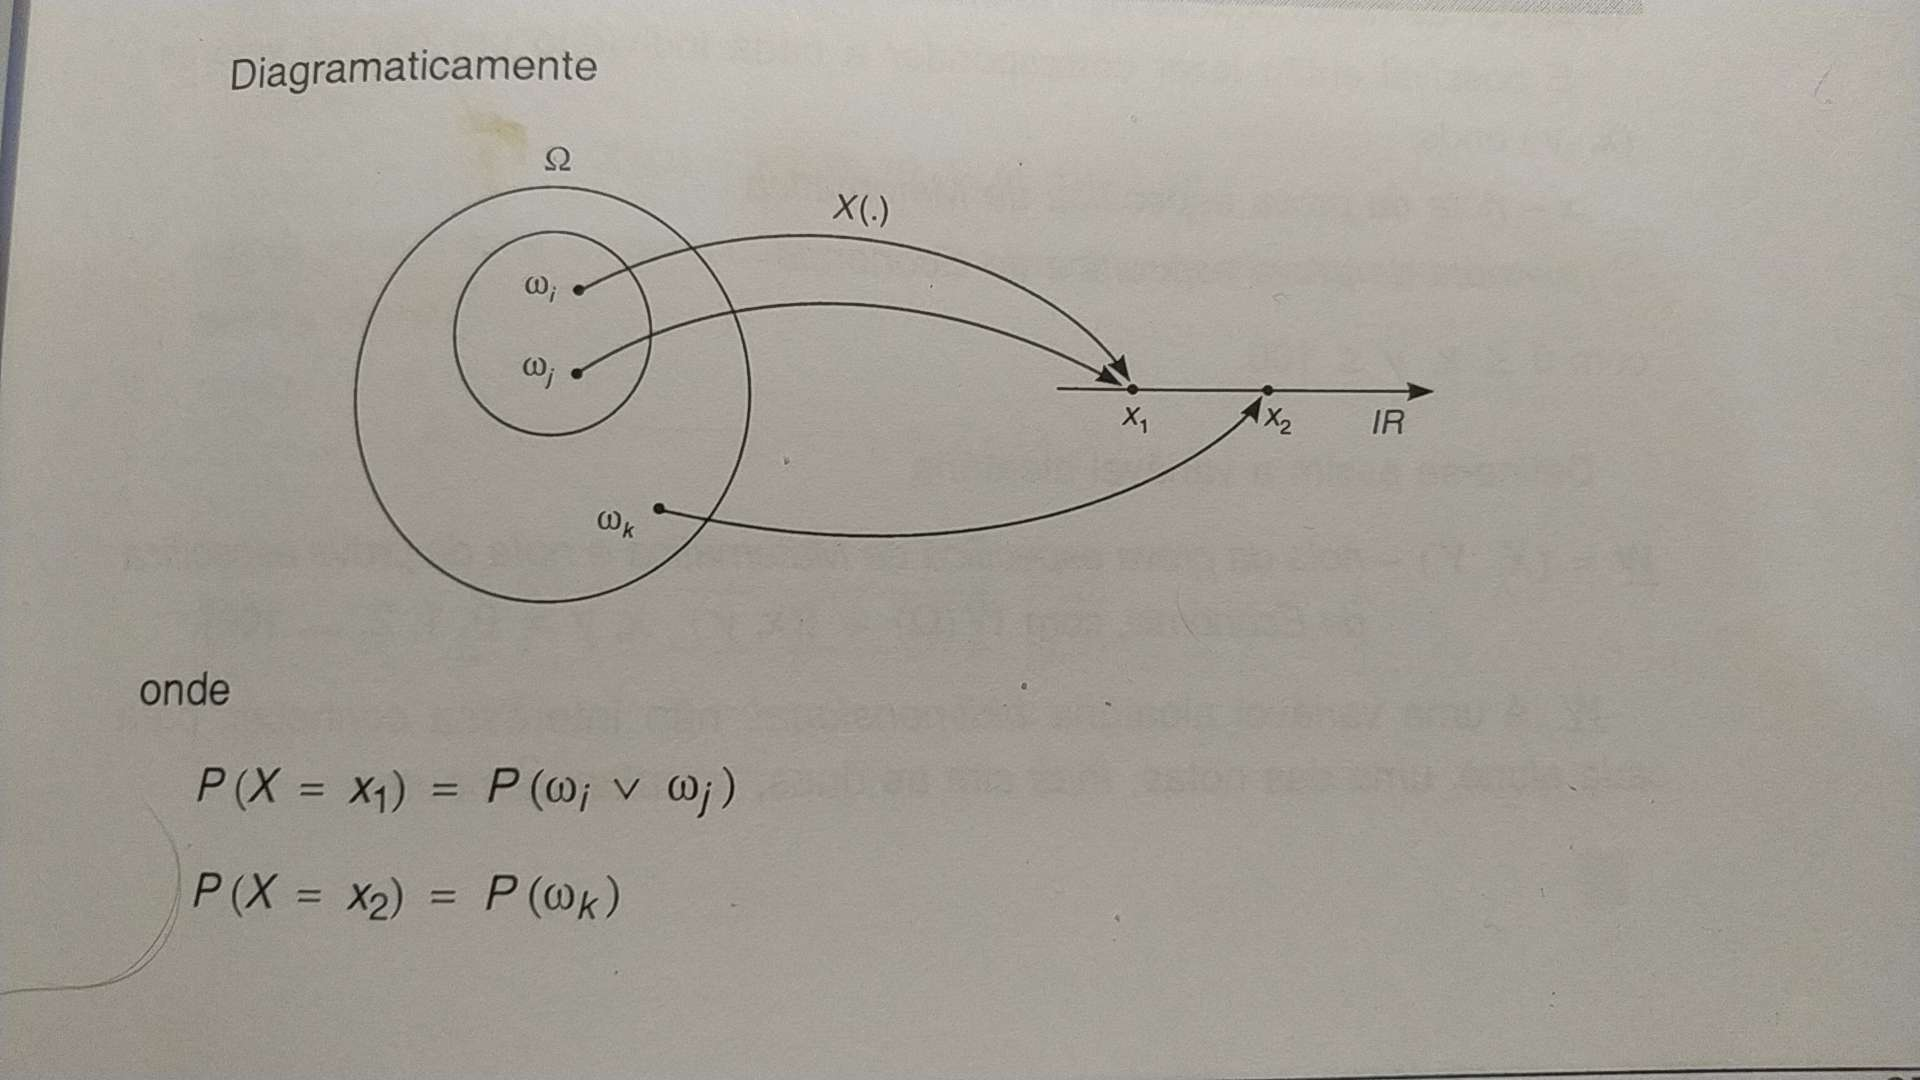
\includegraphics[width=\columnwidth]{variaveisAleatorias.jpg} %TODO mudar para tex (geogebra?)
\begin{tblr}{X l X[2]}\SetRow{m}
  Variável aleatória & $X(\omega)\; \text{ou}\; X$ & Função que cada acontecimento $\omega$ associa um valor real $x = X(\omega)$ \\\SetRow{m}
  CD de uma Variável aleatória & $X(\Omega)$ & 
\end{tblr}
\subsubsection{Função (massa) de probabilidade}
X é discreto
\begin{align*}
  &f(x) = P[X = x] \\
  &0 \leq f(x) \leq 1 \\
  &\sum_{i=1}^n f(x_i) = 1 & \text{caso } n {\text{ finito}} \\
  &\sum_{i=1}^{\infty} f(x_i) = 1 & \text{caso } n {\text{ infinito}} \\
\end{align*}
\subsubsection{Função densidade de probabilidade}
X é contínuo, e é comum a função ser parametrizada (p.e. $f(x;\mu ,\sigma ^{2})$), dependendo da distribuição de X
\begin{align*}
  &f(x) = \frac {d}{dx}F(x) \\
  &0 \leq f(x) \leq 1 \\
  &\int_{-\infty}^{\infty} f(x)/; dx = 1 \\
  &P[X = x] = 0 \; f(x) \neq 0
\end{align*}
\subsubsection{Função de distribuição (acomuldada) (f.d.p.)}
A função é apenas crescente
\begin{align*}
  &F(x) = P[X \leq x] \\
  &0 \leq F(x) \leq 1 \\
  &\forall x_2 > x_1: \\
    &\qquad F(x_2) \geq F(x_1) \\ 
    &\qquad \land F(x_2) - F(x_1) = P[x_1 < X \leq x_2] \\
  &\lim_{x \to -\infty} F(x) = 0 \\ 
  &\lim_{x \to \infty} F(x) = 1 \\
  &P[x_1 < X \leq x_2] = F(x_2) - F(x_1)
\end{align*}
Se $X$ for contínua:
\begin{align*}
  &F(x) = P[X \leq x] = \int_{-\infty}^x f(u) du \\
  &P[x_1 < X \leq x_2] = \int_{x_1}^{x_2} f(u) du
\end{align*}
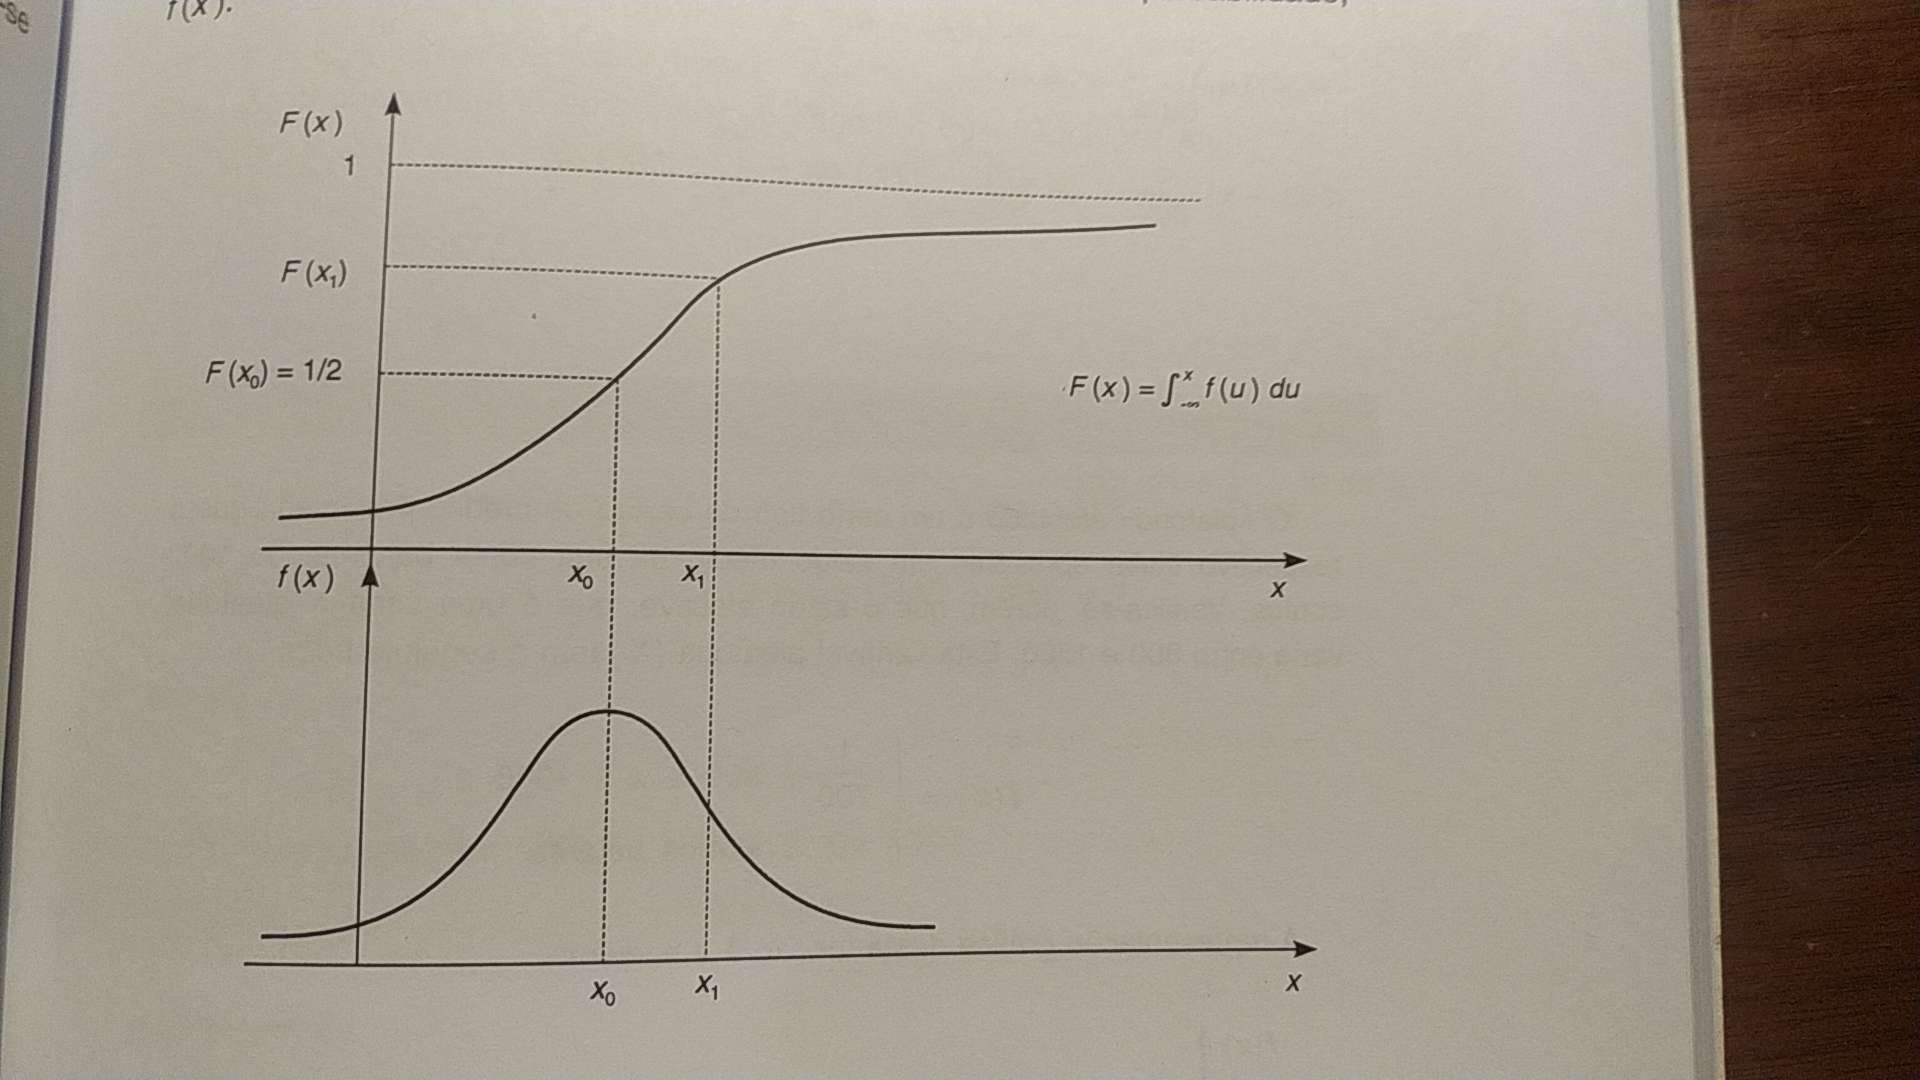
\includegraphics[width=\columnwidth]{fda.jpg} %TODO mudar para tex (geogebra?)
\subsection{Função de probabilidade conjunta}
Se discretas
\begin{align*}
  &f(x, y) = P[X = x, Y = y] = P[X = x \cap Y = y]\\
  &0 \leq f(x, y) \leq 1 \\
  &\sum_{i=1}^n \sum_{j=1}^n f(x_i, y_j) = 1 \\
  &F(x, y) = P[X \leq x, Y \leq y] = \sum_{x_i \leq x} \sum_{y_j \leq y} f(x_i, y_j) \\
  &\lim_{x \to -\infty \land y \to -\infty} F(x, y) = 0 \\
  &\lim_{x \to \infty \land y \to \infty} F(x, y) = 1 \\
  &\forall \lambda \in \mathbb{R}: \\
    &\qquad \lim_{x \to -\infty } F(x, \lambda) = \lim_{y \to -\infty } F(\lambda, y) = 0 \\
  &\forall x_2 > x_1, y_2 > y_1: F(x_2, y_2) \geq F(x_1, y_1) \\
\end{align*}
Se contínuas

\begin{align*}
  &f(x, y) = \frac{\partial^2 F(x, y)}{\partial x \partial y} \\
  &F(x, y) = \int_{-\infty}^x \int_{-\infty}^y f(u, v) dv du \\
\end{align*}

\subsection{Parâmetros de v.a.s}
\subsection{Valor esperado}
O valor esperado de $X$ é igual à média de $X$.
$$E[X] = \mu_X = \mu$$
Se $X$ for discreta:
$$E[X] = \sum_i x_i \cdot f(x_i)$$
Se $X$ for contínua:
$$E[X] = \int x \cdot f(x) dx$$
\subsubsection{Propriedades}
\begin{align*}
  &E[\lambda] = \lambda \\
  &E[\lambda X] = \lambda E[X] \\
  &E[X \pm Y] = E[X] \pm E[Y] \\
  &E[X Y] = E[X] E[Y] \iff \text{se } X \text{ e } Y \text{ forem independentes} \\
  &E[g(X)] = \sum_i g(x_i) \cdot f(x_i) \iff \text{se } X \text{ for discreta} \\
  &E[g(X)] = \int g(x) \cdot f(x) dx \iff \text{se } X \text{ for contínua} \\
  &E[X^2] = \sum_i x_i^2 \cdot f(x_i) \iff \text{se } X \text{ for discreta}
\end{align*}
%TODO finish + organize variancia 
% aqui está apenas o importante para o teste
\subsection{Variância}
\begin{align*}
  &\sigma^2_X = \sigma^2_X = \sigma^2 \\
  &\sigma^2_X = E[(X - E[X])^2] \\
  &\sigma^2_X = E[X^2] - E[X]^2 \\
  &\sigma^2_X = E[X^2] - \mu^2 \\
  &\sigma^2_X = \sum_i (x_i - \mu)^2 \cdot f(x_i) \iff \text{se } X \text{ for discreta} \\
  &\sigma^2_X = \int (x - E[X])^2 \cdot f(x) dx \iff \text{se } X \text{ for contínua} \\
  &\text{Var}(\lambda) = 0 \\
  &\text{Var}(\lambda X) = \lambda^2 \sigma^2_X \\
  &\text{Var}(X \pm Y) = \sigma^2_X + \sigma_Y^2 \pm 2 cov(X, Y) \\
  &\sigma = \sqrt{\sigma^2} \\
  &Cov(X, Y) = E[(X - \mu_X)(Y - \mu_Y)] \\
  &Cov(X, Y) = E[X \cdot Y] - \mu_x \cdot \mu_y \\
  &Cov(X, Y) = 0 \iff X \text{ e } Y \text{ são independentes} \\
\end{align*}
% falta correlação linear mas n é preciso para este teste me thinks
% also falta momentos mas reza
% also desigualdades
Sendo:
$$W = \frac{X - \mu_X}{\sigma}$$,
$E(W) = 0$ e $\sigma_W^2 = 1$.
\section{Distribuições teóricas discretas}
\subsection{Uniforme}
\begin{align*}
  &f(x; N) = \begin{cases}
    \frac{1}{N} & \text{se } x \in \{1, 2, \ldots, N\} \\
    0 & \text{se não}
  \end{cases} \\
  &F(x; N) = \begin{cases}
    0 & \text{se } x < 1 \\
    \frac{x}{N} & \text{se } 1 \leq x \leq N \\
    1 & \text{se } x > N
  \end{cases} \\
  &E[X] = \frac{N + 1}{2} \\
  &\sigma^2_X = \frac{N^2 - 1}{12}
\end{align*}
\subsection{Distribuição de Bernoulli}
A distribuição de Bernoulli é uma distribuição binomial
\begin{align*}
  &f(x; p) = \begin{cases}
    1 - p & \text{se } x = 0 \\
    p & \text{se } x = 1
  \end{cases} \\
  &f(x; p) =  p^x (1 - p)^{1 - x} \\
  &F(x; p) = \begin{cases}
    0 & \text{se } x < 0 \\
    1-p & \text{se } 0 \leq x < 1 \\
    1 & \text{se } x \geq 1
  \end{cases} \\
  &E[X] = p \\
  &\sigma^2_X = p(1 - p)
\end{align*}
\subsection{Distribuição binomial}
$$X \cap (n; p)$$
\begin{align*}
  &f(x; n, p) = \begin{cases}
    \binom{n}{x} p^x (1 - p)^{n - x} & \text{se } x \in \{0, 1, \ldots, N\} \\
    0 & \text{se não}
  \end{cases} \\
  &F(x; n, p) = \begin{cases}
    0 & \text{se } x < 0 \\
    \sum\limits_{i=0}^x \binom{n}{i} p^i (1 - p)^{n - i} & \text{se } 0 \leq x < n \\
    1 & \text{se } x \geq n
  \end{cases} \\
  &E[X] = np \\
  &\sigma^2_X = np(1 - p) \\
  &\sum_{i=1}^k X_i \cap b\left(\sum^k_{i=1} n_i; p\right) \iff X_i \cap (n_i; p) \text{ são independentes}
\end{align*}
\subsection{Processo de Poisson}
$$X \cap \text{p}(\lambda; t)$$
\begin{align*}
  &f(x; \lambda, t) = \begin{cases}
    e^{-t\lambda}\frac{(t\lambda)^x}{x!} & \text{se } x \in \mathbb{N} \\
    0 & \text{se não}
  \end{cases} \\
  &F(x; \lambda, t) = \begin{cases}
    0 & \text{se } x < 0 \\
    e^{-t\lambda} \sum\limits_{i=0}^x \frac{(t\lambda)^i}{i!} & \text{se } 0 \leq x < \infty \\
    1 & \text{se } x \geq \infty
  \end{cases} \\
  &E[X] = t\lambda \\
  &\sigma^2_X = t\lambda \\
  &\sum_{i=1}^k X_i \cap p\left(\sum^k_{i=1} t_i\lambda_i\right) \iff X_i \cap \text{p}(\lambda_i, t_i) \text{ são independentes}
\end{align*}
\subsection{Distribuição de Poisson}
A distribuição de Poisson é um processo de Poisson onde t = 1
$$X \cap \text{p}(\lambda)$$
A distribuição binomial converge para a distribuição de Poisson quando $n \to \infty$ e $p \to 0$, sendo $\lambda = np$ constante.
$$\lim_{n \to \infty} \text{b}(n; p)= \text{p}(\lambda = np)$$
% falta multinomial e binomial negativa e geométrica e hipergeométrica mas n sai
\section{Distribuições teóricas contínuas}
\subsection{Uniforme}
\begin{align*}
  &f(x; a, b) = \begin{cases}
    \frac{1}{b - a} & \text{se } a \leq x \leq b \\
    0 & \text{se } x < a \text{ ou } x > b
  \end{cases} \\
  &F(x; a, b) = \begin{cases}
    0 & \text{se } x < a \\
    \frac{x - a}{b - a} & \text{se } a \leq x \leq b \\
    1 & \text{se } x > b
  \end{cases} \\
  &E[X] = \frac{a + b}{2} \\
  &\sigma^2_X = \frac{(b - a)^2}{12}
\end{align*}
\subsection{Normal}
$X \cap \text{n}(\mu, \sigma)$
\begin{align*}
  &f(x; \mu, \sigma) = \frac{1}{\sigma\sqrt{2\pi}} \cdot \text{exp}\left(-\frac{1}{2}\left(\frac{(x - \mu)}{\sigma}\right)^2\right) \\
  &E[X] = \mu \\
  &\sigma^2_X = \sigma^2
\end{align*}
A normal normalmente transforma-se na normal padrão, com $\mu_Z = 0$ e $\sigma_Z = 1$, onde $Z = \frac{X - \mu_X}{\sigma_X}$.
$F(x) -> \phi(z)$, $ f(x) -> \varphi(z)$ e $F^{-1}(x) -> \phi^{-1}(z)$ (função quartil)
\begin{align*}
  &\varphi(z) = \frac{1}{\sqrt{2\pi}} \cdot \text{exp}\left(-\frac{1}{2}z^2\right) \\
  &P[\mu - \sigma < X < \mu + \sigma] = P[-1 < Z < 1] \approx 0.68 \\
  &P[\mu - 2\sigma < X < \mu + 2\sigma] = P[-2 < Z < 2] \approx 0.95 \\
  &P[\mu - 3\sigma < X < \mu + 3\sigma] = P[-3 < Z < 3] \approx 0.99 \\
  &\phi^{-1}(0.95) = 1.645 \\
  &\phi^{-1}(0.99) = 2.326 % TODO verificar
\end{align*}
Aditividade:
\begin{align*}
  & T = \sum^k_{i=1} X_i \cap \text{n}\left(k \mu; \sigma \sqrt{k}\right) \\ & \qquad \iff X_i \cap \text{n}(\mu, \sigma) \text{ são independentes}\\
  & T = \sum^k_{i=1} a_i X_i \cap \text{n}\left(\sum a_i \mu_i; \sqrt{\sum a_i^2 \sigma_i^2}\right) \\
  & \left(X_1 \pm X_2\right) \cap \text{n}\left(\mu_1 \pm \mu_2; \sqrt{\sigma_1^2 + \sigma_2^2}\right) \\
  & X \aproxcap \text{n}(n p; \sqrt{np(1 - p)}) \iff \\ 
    &\qquad \iff X \cap \text{b}(n, p), n \to \infty, 0.1 < p < 0.9 \\
  & X \aproxcap \text{n}(\lambda; \sqrt{\lambda}) \iff \\ 
  &\qquad \iff X \cap \text{p}(\lambda), \lambda \to \infty
\end{align*}
Em termos práticos, $k \to \infty$ significa $k > 30$
\section{Amostras}
\subsection{Amostras aleatórias}
A variável aleatória $(X_1, X_2, \ldots, X_n)$ é uma amostra aleatória de uma população se:
$$f(x_1, x_2, \ldots, x_n) = \prod(f(x_i))$$
, onde $X_1$ é o primeiro elemento da amostra, $X_2$ o segundo e $X_n$ o n-ésimo. \\
Cada estatística (amostral) é uma variável aleatória
 \begin{align*}
  &\overline{X} = \frac{1}{n} \sum^n_{i=1} X_i & \text{Média amostral} \\
  &S^2 = \frac{1}{n} \sum^n_{i=1} \left(X_i - \overline{X}\right)^2 & \text{Variância amostral} \\
  &S^{'2} = \frac{1}{n - 1} \sum^n_{i=1} \left(X_i - \overline{X}\right)^2 & \text{Variância amostral corrigida}
\end{align*}
\subsection{Teorema do limite central}
\begin{flalign*}
  &\frac{\sum \left(X_i\right) - n \mu}{\sigma\sqrt{n}} \aproxcap \text{n}(0, 1)&& \\
  &\sum{X_i} \aproxcap \text{n}\left(n\mu, \sigma\sqrt{n}\right)&& \\
  &\text{Como } \frac{\sum{X_i}}{n} = \overline{X}: &&\\
    &\qquad \overline{X} \aproxcap \text{n}\left(\mu, \frac{\sigma}{\sqrt{n}}\right)&&
\end{flalign*}
Se e apenas se:
\begin{flalign*}
  &E[X_1] = E[X_2] = \ldots = E[X_n] = \mu, && \\
  &\text{Var}[X_1] = \text{Var}[X_2] = \ldots = \text{Var}[X_n] = \sigma^2, && \\
  &n \to \infty. &&
\end{flalign*}
% TODO falta t student e a outra q ainda n percebi o q sai disso
\subsection{Distribuições de amostras de populações}
\subsubsection{Populações Bernoulli}
\begin{align*}
  \overline{X} &\aproxcap \text{n}\left(p, \sqrt{\frac{pq}{n}}\right) \\
  \left(\overline{X_1} - \overline{X_2}\right) &\aproxcap \text{n}\left(p_1 - p_2, \sqrt{\frac{p_1 q_1}{n_1} + \frac{p_2 q_2}{n_2}}\right) \\
\end{align*}
\subsubsection{Populações normais}
\begin{align*}
  &\text{quando } \sigma^2 \text{ é conhecida:} \\
    &\qquad \overline{X} \aproxcap \text{n}\left(\mu, \frac{\sigma}{\sqrt{n}}\right) \\
  &\text{quando } \sigma^2 \text{ é desconhecida:} \\
    &\qquad \frac{\overline{X} - \mu}{\frac{S'}{\sqrt{n}}} \aproxcap \text{t}_{n-1} \\
  &\frac{(n-1)S^{'2}}{\sigma^2} \aproxcap \chi^2_{n-1} \\
  &\frac{n S^2}{\sigma^2} \aproxcap \chi^2_{n-1} \\
  &\overline{X_1} - \overline{X_2} \cap \text{n}\left(\mu_1 - \mu_2, \sqrt{\frac{\sigma_1^2}{n_1} + \frac{\sigma_2^2}{n_2}}\right) \\
  &\overline{X_1} - \overline{X_2} \aproxcap \text{n}\left(\mu_1 - \mu_2, \sqrt{\frac{S_1^{'2}}{n_1} + \frac{S_2^{'2}}{n_2}}\right)
\end{align*}
\section{temp}
\blinddocument
\end{multicols}
\end{document}
